\chapter{Problemi intrattabili e teoria dell'NP-completezza}
\section{Introduzione}
Finora, con l'unica eccezione della sezione sul \emph{backtracking}, abbiamo
trattato unicamente problemi con soluzioni in tempo \emph{polinomiale}, ovvero
problemi le cui soluzioni sono eseguibili in tempo $O(n^k)$ con $k\in\mathbb{R}^+$.
Esistono anche problemi che richiedono un tempo \emph{esponenziale} o che
addirittura non sono risolvibili (e.g. halting problem).

Ciò che andremo ad introdurre in questo capitolo invece, sono una serie di
problemi per i quali non è chiaro se esista o meno una soluzione
\emph{polinomiale}. Vedremo anche come tutti questi problemi siano in realtà
legati tra loro, in modo che se esiste una soluzione \emph{polinomiale} per uno
di essi, allora ne esiste una anche per gli altri. Viceversa, se si riesce a
dimostrare che uno di essi non è risolvibile in tempo \emph{polinomiale}, allora
non lo è nessuno.

\bigskip\noindent
Procediamo dando alcune definizioni.

\begin{definition}[Problema astratto]
    Un problema astratto è una relazione binaria $R\subseteq I\times S$ tra un
    insieme $I$ di istanze del problema e un insieme $S$ di soluzioni.
\end{definition}
\begin{note}
    Ad esempio, nel problema della \emph{ricerca del cammino minimo tra due
    nodi}, un'istanza del problema è la tupla $(V,R,u,v)$, mentre una soluzione
    è una sequenza di \emph{nodi} $(v_1,\dots,v_n)$.
\end{note}

\noindent
Come visto nei capitoli scorsi, esistono varie tipologie di problema. Le
principali sono tre: \emph{ottimizzazione}, \emph{ricerca} e \emph{decisione}.

\begin{definition}[Problema di ottimizzazione]
    Data un'istanza, trovare la soluzione ottima secondo un insieme di criteri
    prestabiliti.
\end{definition}
\begin{definition}[Problema di ricerca]
    Data un'istanza, trovare una possibile soluzione tra quelle esistenti.
\end{definition}
\begin{definition}[Problema di decisione]
    Data un'istanza, verificare se soddisfa o meno una data proprietà.
\end{definition}
\begin{note}
    Nei \emph{problemi di decisione}, $R$ è una funzione del tipo $R:I\to\{0,1\}$.
\end{note}

\noindent
Informalmente, possiamo dimostrare che i \emph{problemi di ottimizzazione} e di
\emph{decisione} sono equivalenti.

\begin{proof}[Dimostrazione]
    Se è possibile risolvere efficientemente un \emph{problema di ottimizzazione},
    allora è possibile usare la soluzione a quel problema per verificare
    efficientemente la proprietà interessata dal \emph{problema di decisione}
    associato.

    Da questa affermazione possiamo derivare la seguente: se non è possibile
    risolvere efficientemente un \emph{problema di decisione}, allora non è
    nemmeno possibile risolvere efficientemente il \emph{problema di
    ottimizzazione} associato.
\end{proof}
\begin{note}
    Ad esempio, nel problema della \emph{ricerca del cammino tra due nodi}, se
    si conosce il \emph{cammino minimo} tra essi, è possibile risolvere
    efficientemente un \emph{problema di decisione} nel quale ci si chiede se
    esista un \emph{cammino} di lunghezza non superiore a un qualche valore $k$.
\end{note}

\noindent
Questa dimostrazione, sebbene informale, ci permette di proseguire la trattazione
concentrandoci unicamente su \emph{problemi decisionali}, che sono più facili sia
da definire che da elaborare.

\section{Riduzioni}
\begin{definition}[Riduzione polinomiale]
    Dati due problemi decisionali $R_1\subseteq I_1\times\{0,1\}$ e
    $R_2\subseteq I_2\times\{0,1\}$, diciamo che $R_1$ è riducibile
    polinomialmente a $R_2$, e scriviamo in simboli $R_1\leq_p R_2$, se esiste
    una funzione $f:I_1\to I_2$ che sia calcolabile in tempo polinomiale e tale
    per cui, per ogni istanza $x$ del problema $R_1$ e ogni soluzione $s\in\{0,1\}$,
    sia vero che $(x,s)\in R_1\Leftrightarrow(f(x), s)\in R_2$.
\end{definition}

\begin{figure}[h!]
\centering
\scalebox{1}{\begin{graph}
    \definecolor{pink}{RGB}{255, 204, 204}
    \definecolor{yellow}{RGB}{255, 251, 214}
    \tikzset{
        cell/.style={fill=pink, draw, rectangle, minimum size=12mm, inner sep=0},
        bg/.style={fill=yellow, draw, rectangle, inner sep=0, minimum size=20mm}
    }
    
    \node[bg] (1) [minimum width=70mm, label={[yshift=7mm]-90:{$A_1$}}] {};
    \node[cell] (f) at (1) [xshift=-25mm] {$f$};
    \node[cell] (a2) at (1) [xshift=25mm] {$A_2$};

    \node[] (0) at (f) [xshift=-35mm] {};
    \node[] (1) at (a2) [xshift=35mm] {};

    \draw[->]   (f) edge node[above] {$f(x)\in I_2$} (a2);
    \draw[->]   (0) edge node[above] {$x\in I_1$} (f);
    \draw[->]   (a2) edge node[above] {$s\in\{0,1\}$} (1);
\end{graph}}
\caption{\emph{Riduzione polinomiale}}
\end{figure}

\noindent
Proseguiamo la trattazione con una carrellata di problemi che, vedremo,
possono essere legati tra loro mediante \emph{riduzioni polinomiali}.

\subsection{Colorazione di grafi}
\begin{definition}[Colorazione di grafi]
    Dati un grafo non orientato $G=(V,E)$ e un insieme di colori $C$, una
    colorazione dei vertici è una funzione $f:V\to C$ che assegna ad ogni nodo
    uno dei colori in $C$ in maniera tale per cui nessuna coppia di nodi adiacenti
    ha lo stesso colore
\end{definition}
\begin{problem}[Colorabilità di un grafo (GRAPH-COLORING)]
    Dato un grafo non orientato $G=(V,E)$ e un valore $k$, determinare se
    esiste una colorazione di $G$ con $k$ colori.
\end{problem}

\subsection{Sudoku}
\begin{problem}[Risolvibilità di un sudoku (SUDOKU)]
    Data una matrice $n^2\times n^2$ con alcuni numeri già inseriti, determinare
    se esiste un modo per assegnare i numeri restanti in modo coerente con le
    regole dei Sudoku.
\end{problem}

\noindent
Il problema sulla \emph{risolvibilità di un sudoku} può essere \emph{ridotto
polinomialmente} al problema sulla \emph{colorabilità di un grafo}. In
particolare, è possibile tradurre la matrice del sudoku in un \emph{grafo} in
cui ogni valore della matrice diventa un \emph{nodo} del \emph{grafo} e in cui
tra due \emph{nodi} esiste un \emph{arco} soltanto se, all'interno della matrice,
quei \emph{nodi} sono sulla stessa riga, sulla stessa colonna o sulla stessa
diagonale. Formalmente gli insiemi dei \emph{nodi} e degli \emph{archi} sono
definiti come segue:
\[V=\left\{(x,y):1\leq x\leq n^2, 1\leq y\leq n^2\right\}\]
\[E=\left\{[(x,y),(x',y')]: x=x' \vee y=y' \vee \left(
    \left\lceil\frac{x}{n}\right\rceil =
    \left\lceil\frac{x'}{n}\right\rceil \wedge
    \left\lceil\frac{y}{n}\right\rceil = \left\lceil\frac{y'}{n}\right\rceil
\right)\right\}\]
L'insieme dei colori è $C=\{1,\dots,n\}$.

\begin{figure}[h!]
\centering

\resizebox*{0.98\textwidth}{!}{
    \begin{graph}
        \definecolor{r}{rgb}{0.9, 0.17, 0.31}
        \definecolor{y}{rgb}{0.93, 0.53, 0.18}
        \definecolor{g}{rgb}{0, 0.42, 0.24}
        \definecolor{b}{rgb}{0, 0, 0 0}
        \definecolor{lavendergray}{rgb}{0.77, 0.76, 0.82}
        \def\numbers{%
            1 2 3 4
            3 4 1 2
            2 3 4 1
            4 1 2 3
        }
        \readarray\numbers\num[4,4]
        \def\colors{%
            r y g b
            g b r y
            y b b r
            b r y g
        }
        \readarray\colors\col[4,4]

        \tikzset{
          noder/.style={circle, draw, minimum size=5mm, fill=r},
          nodey/.style={circle, draw, minimum size=5mm, fill=y},
          nodeg/.style={circle, draw, minimum size=5mm, fill=g},
          nodeb/.style={circle, draw, minimum size=5mm, fill=b},
          empty/.style={inner sep=0em, minimum size=10mm},
          cell/.style={rectangle, draw=lavendergray, minimum size=10mm, font=\large},
          square/.style={rectangle, draw, minimum size=20mm},
          node distance=15mm
        }

        \foreach \x in {1,...,4}
            \foreach \y in {1,...,4}
            {
                \node[cell] (m\x\y) at (\x-1,-\y-1) [text={\col[\y,\x]}] {$\num[\y,\x]$};
            }

        \node[square] (q1) at (m11) [xshift=5mm, yshift=-5mm, label=above left:{$A$}] {};
        \node[square] (q2) at (m13) [xshift=5mm, yshift=-5mm, label=below left:{$C$}] {};
        \node[square] (q3) at (m31) [xshift=5mm, yshift=-5mm, label=above right:{$B$}] {};
        \node[square] (q4) at (m33) [xshift=5mm, yshift=-5mm, label=below right:{$D$}] {};

        \node[empty] (arrow) [right of=m43, yshift=5mm] {$\Longrightarrow$};
        \node[empty] (0) [right of=arrow, xshift=55mm] {};
        \node[empty] (w) [left of=0, xshift=-25mm] {};
        \node[empty] (e) [right of=0, xshift=25mm] {};
        \node[empty] (s) [below of=0, yshift=-25mm] {};
        \node[empty] (n) [above of=0, yshift=25mm] {};

        \node[nodeg] (w1) [above of=w] {};
        \node[nodey] (w2) [above left of=w, yshift=-5mm] {};
        \node[noder] (w3) [below left of=w, yshift=5mm] {};
        \node[nodeb] (w4) [below of=w] {};

        \node[noder] (n1) [left of=n] {};
        \node[nodey] (n2) [above left of=n, xshift=5mm] {};
        \node[nodeg] (n3) [above right of=n, xshift=-5mm] {};
        \node[nodeb] (n4) [right of=n] {};

        \node[nodeg] (e1) [above of=e] {};
        \node[nodeb] (e2) [above right of=e, yshift=-5mm] {};
        \node[noder] (e3) [below right of=e, yshift=5mm] {};
        \node[nodey] (e4) [below of=e] {};

        \node[nodey] (s1) [right of=s] {};
        \node[nodeg] (s2) [below right of=s, xshift=-5mm] {};
        \node[nodeb] (s3) [below left of=s, xshift=5mm] {};
        \node[noder] (s4) [left of=s] {};

        % Archi tra nodi della stessa matrice nxn: solo archi dritti
        \path[-]    (w1) edge (w2)
                    (w2) edge (w3)
                    (w3) edge (w4)
                    (n1) edge (n2)
                    (n2) edge (n3)
                    (n3) edge (n4)
                    (e1) edge (e2)
                    (e2) edge (e3)
                    (e3) edge (e4)
                    (s1) edge (s2)
                    (s2) edge (s3)
                    (s3) edge (s4);

        \path[-, bend right=10]
                    (w3) edge (w1)
                    (w4) edge (w1)
                    (w4) edge (w2)
                    (n1) edge (n3)
                    (n1) edge (n4)
                    (n2) edge (n4)
                    (e1) edge (e3)
                    (e1) edge (e4)
                    (e2) edge (e4)
                    (s1) edge (s3)
                    (s1) edge (s4)
                    (s2) edge (s4);

        \path[-, bend right=10]
                    (w1) edge (n4)
                    (n4) edge (e4)
                    (e4) edge (s4)
                    (s4) edge (w1)
                    (w2) edge (n3)
                    (n3) edge (e3)
                    (e3) edge (s3)
                    (s3) edge (w2)
                    (w3) edge (n2)
                    (n2) edge (e2)
                    (e2) edge (s2)
                    (s2) edge (w3)
                    (w4) edge (n1)
                    (n1) edge (e1)
                    (e1) edge (s1)
                    (s1) edge (w4);

        % Archi orizzontanti e verticali
        \path[-]    (w1) edge (e4)
                    (w2) edge (e3)
                    (w3) edge (e2)
                    (w4) edge (e1)
                    (n1) edge (s1)
                    (n2) edge (s2)
                    (n3) edge (s3)
                    (n4) edge (s4);

        \draw[-] (w1)+(0,5mm) arc(90:270:1.5cm and 2cm) node[midway, left] {$D$};
        \draw[-] (n1)+(-5mm,0) arc(180:0:2cm and 1.5cm) node[midway, above] {$A$};
        \draw[-] (e1)+(0,5mm) arc(90:270:-1.5cm and 2cm) node[midway, right] {$B$};
        \draw[-] (s1)+(5mm,0) arc(0:180:2cm and -1.5cm) node[midway, below] {$C$};
    \end{graph}
}
\caption{Trasformazione \emph{matrice-grafo}}
\end{figure}

\noindent
Questo significa che $\text{SUDOKU}\leq_p\text{GRAPH-COLORING}$, quindi una
soluzione al problema della colorazione può essere usata per risolvere il
problema del sudoku.

\subsection{Insieme indipendente}
\begin{definition}[Insieme indipendente]
    Dato un grafo non orientato $G=(V,E)$, un insieme $S\subseteq V$ è un insieme
    indipendente se e solo se nessun arco in $E$ unisce due nodi in $S$. Ovvero,
    $S$ è un insieme indipendente se vale la seguente relazione:
    \[x\notin S\vee y\notin S\quad\forall(x,y)\in E\]
\end{definition}
\begin{problem}[Esistenza di un insieme indipendente (INDIPENDENT-SET)]
    Dati un grafo non orientato $G=(V,E)$ e un valore $k$, dire se esiste un
    insieme indipendente di dimensione almeno $k$.
\end{problem}

\begin{figure}[h!]
    \centering
    \begin{graph}
        \node[main] (a) [line width=1.3pt] {$a$};
        \node[main] (c) [below right of=a] {$c$};
        \node[main] (b) [above right of=c] {$b$};
        \node[main] (d) [below left of=c] {$d$};
        \node[main] (e) [below right of=c, line width=1.3pt] {$e$};

        \node[] (S) [right of=c, xshift=20mm] {$S=\{a,e\}$};

        \path[-]    (a) edge (b)
                    (a) edge (c)
                    (a) edge (d)
                    (b) edge (e)
                    (b) edge (c)
                    (c) edge (d)
                    (c) edge (e)
                    (d) edge (e);
    \end{graph}
    \caption{Esempio di \emph{insieme indipendente} di dimensione $k=2$}
\end{figure}
\begin{note}
    In questo esempio, avremmo anche potuto scegliere $S=\{b,d\}$.
\end{note}

\subsection{Copertura di vertici}
\begin{definition}[Copertura di vertici]
    Dato un grafo non orientato $G=(V,E)$, un insieme $S\subseteq V$ è una
    copertura di vertici se e solo se ogni arco in $E$ ha almeno un vertice in
    $S$. Ovvero, $S$ è una copertura di vertici se vale la seguente relazione:
    \[x\in S\vee y\in S\quad\forall(x,y)\in E\]
\end{definition}
\begin{problem}[Esistenza di una copertura di vertici (VERTEX-COVER)]
    Dati un grafo non orientato $G=(V,E)$ e un valore $k$, dire se esiste una
    copertura di vertici di dimensione al massimo $k$.
\end{problem}

\begin{figure}[h!]
    \centering
    \begin{graph}
        \node[main] (a) {$a$};
        \node[main] (c) [below right of=a, line width=1.3pt] {$c$};
        \node[main] (b) [above right of=c, line width=1.3pt] {$b$};
        \node[main] (d) [below left of=c, line width=1.3pt] {$d$};
        \node[main] (e) [below right of=c] {$e$};

        \node[] (S) [right of=c, xshift=20mm] {$S=\{b,c,d\}$};

        \path[-]    (a) edge (b)
                    (a) edge (c)
                    (a) edge (d)
                    (b) edge (e)
                    (b) edge (c)
                    (c) edge (d)
                    (c) edge (e)
                    (d) edge (e);
    \end{graph}
    \caption{Esempio di \emph{copertura di vertici} di dimensione $k=3$}
\end{figure}
\begin{note}
    In questo esempio, avremmo anche potuto scegliere $S=\{a,c,e\}$.
\end{note}

\noindent
Dagli ultimi due esempi fatti risulta particolarmente evidente il legame di
dualità che sussiste tra un \emph{insieme indipendente} e una \emph{copertura
di vertici} di uno stesso \emph{grafo}. Infatti, se $S\subseteq V$ è un
\emph{insieme indipendente}, $V-S$ è una \emph{copertura di vertici}, e viceversa.

\bigskip\noindent
La dimostrazione di quanto detto è banale:
\begin{proof}[Dimostrazione]
    Dimostriamo separatamente le due implicazioni:

    \paragraph{\bm{$S$} insieme indipendente \bm{$\Rightarrow$} \bm{$V-S$}
    copertura di vertici}
    Se $S$ è un \emph{insieme indipendente}, per definizione, non esistono
    \emph{archi} $(x,y)\in E$ che abbiano entrambi i \emph{vertici} in $S$.
    Di conseguenza, almeno uno dei due \emph{vertici} deve appartenere a $V-S$.

    \paragraph{\bm{$V-S$} copertura di vertici \bm{$\Rightarrow$} \bm{$S$}
    insieme indipendente}
    Se supponiamo per assurdo che $S$ non sia un \emph{insieme indipendente},
    allora dovrebbe esistere un \emph{arco} $(x,y)$ tale per cui $x,y\in S$.
    Se così fosse però, né $x$, né $y$ apparterrebbero a $V-S$ e quindi $V-S$
    non potrebbe essere una \emph{copertura di vertici}, generando un assurdo.
\end{proof}

\noindent
Con questa dimostrazione abbiamo dimostrato che i due problemi sono equivalenti,
e quindi valgono le seguenti relazioni di \emph{riducibilità polinomiale}:
\[\text{VERTEX-COVER}\leq_p\text{INDIPENDENTE-SET}\]
\[\text{INDIPENDENTE-SET}\leq_p\text{VERTEX-COVER}\]

\subsection{Soddisfacibilità di formule booleane}
\begin{definition}[Forma normale congiuntiva per formule booleane]
    Dato un insieme $V$ contenente $n$ variabili booleane si definisce letterale
    una variabile $v$ o il suo negato $\bar{v}$. Una disgiunzione di letterali,
    ovvero un insieme di letterali separati dall'operatore \bc{or}, costituisce
    una clausola. Infine, una formula booleana si dice essere in forma normale
    congiuntiva se è costituita da una congiunzione di clausole, ovvero da un
    insieme di clausole separate dall'operatore \bc{and}.
\end{definition}
\begin{problem}[Soddisfacibilità di formule booleane (SAT)]
    Data un'espressione in forma normale congiuntiva, stabilire se esiste
    un'assegnazione di valori di verità alle variabili che renda vera l'espressione.
\end{problem}
\begin{eg}[Esempio]
    Se $V=\{w,x,y,z\}$ e l'espressione da valutare è la seguente:
    \[(x\vee\bar{y}\vee z)\wedge(\bar{x}\vee w)\wedge y\]
    Alcune assegnazioni che rendono vera l'espressione sono:
    \begin{itemize}
        \item $w=x=y=z=\bc{true}$;
        \item $w=x=y=\bc{true}$, $z=\bc{false}$;
    \end{itemize}
\end{eg}
\begin{problem}[Soddisfacibilità di formule booleane con 3 letterali (3-SAT)]
    Data un'espressione in forma normale congiuntiva in cui ciascuna clausola ha
    esattamente 3 letterali, stabilire se esiste un'assegnazione di valori di
    verità alle variabili che renda vera l'espressione.
\end{problem}

\noindent
Ciò che vogliamo fare ora è dimostrare che $\text{3-SAT}\leq_p\text{INDIPENDENT-SET}$.
Per farlo, \emph{riduciamo polinomialmente} 3-SAT a INDIPENDENT-SET trasformando
l'espressione booleana in un \emph{grafo}, nel quale, per ogni \emph{clausola}
viene aggiunto un trio di \emph{nodi} collegati tra loro da \emph{archi}.
Inoltre, viene aggiunto un \emph{arco} anche tra ogni \emph{letterale} e il
suo negato.

\bigskip\noindent
Ad esempio, il \emph{grafo} associato all'espressione $(x\vee\bar{y}\vee z)\wedge
(\bar{x}\vee\bar{y}\vee\bar{z})\wedge(\bar{x}\vee y\vee z)$ è il seguente:
\begin{figure}[h!]
    \centering
    \begin{graph}
        \node[main] (x1) {$x$};
        \node[main] (z1) [above right of=x1, yshift=5mm] {$z$};
        \node[main] (y1) [below right of=z1, yshift=-5mm] {$\bar{y}$};

        \node[main] (x2) [right of=y1, xshift=5mm] {$\bar{x}$};
        \node[main] (z2) [above right of=x2, yshift=5mm] {$\bar{z}$};
        \node[main] (y2) [below right of=z2, yshift=-5mm] {$\bar{y}$};

        \node[main] (x3) [right of=y2, xshift=5mm] {$\bar{x}$};
        \node[main] (z3) [above right of=x3, yshift=5mm] {$z$};
        \node[main] (y3) [below right of=z3, yshift=-5mm] {$y$};

        \path[-]    (x1) edge (y1)
                    (x1) edge (z1)
                    (z1) edge (y1)
                    (x2) edge (y2)
                    (x2) edge (z2)
                    (z2) edge (y2)
                    (x3) edge (y3)
                    (x3) edge (z3)
                    (z3) edge (y3);
        \path[-, bend left=20]
                    (z1) edge (z2)
                    (z2) edge (z3)
                    (y3) edge (y2)
                    (y3) edge (y1)
                    (x3) edge (x1)
                    (x2) edge (x1);
    \end{graph}
    \caption{\emph{Grafo} associato a una formula 3-SAT}
\end{figure}

\noindent
Costruito il \emph{grafo}, la formula è soddisfacibile se e solo se è possibile
trovare un \emph{insieme indipendente} composto da tanti elementi quante sono
le \emph{clausole} dell'espressione booleana.

\bigskip\noindent
Nell'esempio che stiamo considerando, la soluzione è la seguente:

\begin{figure}[h!]
    \centering
    \begin{graph}
        \node[main] (x1) [line width=1.3pt] {$x$};
        \node[main] (z1) [above right of=x1, yshift=5mm] {$z$};
        \node[main] (y1) [below right of=z1, yshift=-5mm] {$\bar{y}$};

        \node[main] (x2) [right of=y1, xshift=5mm] {$\bar{x}$};
        \node[main] (z2) [above right of=x2, yshift=5mm] {$\bar{z}$};
        \node[main] (y2) [below right of=z2, yshift=-5mm, line width=1.3pt] {$\bar{y}$};

        \node[main] (x3) [right of=y2, xshift=5mm] {$\bar{x}$};
        \node[main] (z3) [above right of=x3, yshift=5mm, line width=1.3pt] {$z$};
        \node[main] (y3) [below right of=z3, yshift=-5mm] {$y$};

        \path[-]    (x1) edge (y1)
                    (x1) edge (z1)
                    (z1) edge (y1)
                    (x2) edge (y2)
                    (x2) edge (z2)
                    (z2) edge (y2)
                    (x3) edge (y3)
                    (x3) edge (z3)
                    (z3) edge (y3);
        \path[-, bend left=20]
                    (z1) edge (z2)
                    (z2) edge (z3)
                    (y3) edge (y2)
                    (y3) edge (y1)
                    (x3) edge (x1)
                    (x2) edge (x1);
    \end{graph}
    \caption{Possibile soluzione}
\end{figure}
\noindent
L'insieme che abbiamo individuato ci dice quali \emph{letterali} devono
essere posti a \texttt{true}.

\paragraph{Relazione tra SAT, 3-SAT e INDIPENDENT-SET}
Ovviamente $\text{3-SAT}\leq_p\text{SAT}$ perché il primo è un caso particolare
del secondo. Tuttavia, è possibile dimostrare anche la relazione inversa, in
quanto, ogni espressione SAT può essere trasformata in una 3-SAT applicando delle
semplici trasformazioni:
\begin{itemize}
    \item Se la \emph{clausola} è contiene più di 3 \emph{letterali}, si
    introduce una nuova variabile e si spezza la precedente \emph{clausola}:
    \[(a\vee b\vee c\vee d)\equiv(a\vee b\vee z)\wedge(\bar{z}\vee c\vee d)\]
    \item Se la \emph{clausola} è contiene meno di 3 \emph{letterali}, si fa
    il \q{padding}, ovvero si ripete più volte uno stesso \emph{letterale}
    all'interno della stessa \emph{clausola}:
    \[(a\vee b)\equiv(a\vee a\vee b)\]
\end{itemize}

\noindent
Riassumendo i rapporti di \emph{riducibilità polinomiale} riscontrati finora,
otteniamo la seguente catena:
\[\text{SAT}\leq_p\text{3-SAT}\leq_p\text{INDIPENDENT-SET}\leq_p\text{VERTEX-COVER}\]

\section{Classi di problemi}
\begin{definition}[Algoritmo]
    Dati un problema decisionale $R$ e un algoritmo $A$ (scritto in un modello
    di calcolo Turing-equivalente) che lavora in tempo $f_t(n)$ e spazio $f_s(n)$,
    diciamo che $A$ risolve $R$ se restituisce una soluzione $s$ su un'istanza
    $x$ se e solo se $(x,s)\in R$.
\end{definition}
\begin{definition}[Classi di complessità]
    Data una qualunque funzione $f(n)$, chiamiamo $\mathbb{TIME}(f(n))$ e
    $\mathbb{SPACE}(f(n))$ l'insieme dei problemi decisionali risolvibili da un
    algoritmo che lavora rispettivamente in tempo e spazio $O(f(n))$.
\end{definition}
\begin{definition}[Classe $\mathbb{P}$]
    La classe $\mathbb{P}$ comprende tutti i problemi decisionali che sono
    risolvibili in tempo polinomiale rispetto alla dimensione $n$ dell'istanza
    d'ingresso. Ovvero, l'insieme $\mathbb{P}$ è definito come:
    \[\mathbb{P}=\bigcup_{c=0}^{+\infty}\mathbb{TIME}(n^c)\]
\end{definition}
\begin{definition}[Classe $\mathbb{PSPACE}$]
    La classe $\mathbb{PSPACE}$ comprende tutti i problemi decisionali che sono
    risolvibili in spazio polinomiale rispetto alla dimensione $n$ dell'istanza
    d'ingresso. Ovvero, l'insieme $\mathbb{PSPACE}$ è definito come:
    \[\mathbb{PSPACE}=\bigcup_{c=0}^{+\infty}\mathbb{SPACE}(n^c)\]
\end{definition}
\begin{note}
    La \emph{classe} $\mathbb{P}$ è un sottoinsieme della \emph{classe}
    $\mathbb{PSPACE}$, ovvero $\mathbb{P}\subseteq\mathbb{PSPACE}$.
\end{note}

\begin{definition}[Certificato]
    Dati un problema decisionale $R$ e un'istanza $x$ di input tale per cui
    $(x,\bc{true})\in R$, un certificato è un insieme di informazioni che
    permette provare che $(x,\bc{true})\in R$.
\end{definition}

\noindent
Ad esempio, nel problema SAT, un \emph{certificato} è un assegnamento di
valori di verità alle variabili della formula, in GRAPH-COLORING è un'associazione
\emph{nodo-colore} $f:V\to C$ e in INDIPENDENT-SET è un sottoinsieme $S\subseteq V$
di $k$ elementi.
\begin{note}
    Tutti questi \emph{certificati} hanno dimensione \emph{polinomiale}
    rispetto alla dimensione dell'input.
\end{note}

\noindent
È facile convincersi che la verifica di tutti i \emph{certificati} citati sia
possibile in tempo \emph{polinomiale} e questa caratteristica è distintiva dei
problemi appartenenti alla \emph{classe} $\mathbb{NP}$.

\begin{definition}[Classe $\mathbb{NP}$]
    La classe $\mathbb{NP}$ comprende tutti i problemi decisionali che ammettono
    un certificato verificabile in tempo polinomiale.
\end{definition}
\begin{note}
    Non è detto che tutti i \emph{certificati} siano verificabili in tempo
    \emph{polinomiale}.
\end{note}

\begin{definition}[Trasitività dell'appartenenza alla classe $\mathbb{P}$]
    Dati due problemi decisionali $R_1$ e $R_2$ tali per cui $R_1\leq_p R_2$,
    se $R_2\in\mathbb{P}$ allora anche $R_1\in\mathbb{P}$.
\end{definition}
\begin{proof}[Dimostrazione]
    Sia $T_f(n)=O(n^{k_f})$ il tempo necessario per trasformare un input di $R_1$
    in un input di $R_2$ tramite una funzione $f$ e sia $T_2(n)=O(n^{k_2})$ il
    tempo necessario per risolvere $R_2$.

    Poiché la funzione $f$ può prendere un input di dimensione $n$ e trasformarlo
    in un input di dimensione $O(n^{k_f})$ per $R_2$, il tempo necessario per
    risolvere $R_1$ attraverso $R_2$ è $T_1(n)=O(n^{k_fk_2})$ che è un
    tempo \emph{polinomiale}.
\end{proof}

\begin{definition}[Problema $\mathbb{NP}$-arduo]
    Un problema decisionale $R$ si dice essere $\mathbb{NP}$-arduo se
    ogni problema $Q\in\mathbb{NP}$ è riducibile polinomialmente ad $R$, ovvero
    se $Q\leq_p R\quad\forall Q\in\mathbb{NP}$.
\end{definition}
\begin{definition}[Problema $\mathbb{NP}$-completo]
    Un problema decisionale $R$ si dice essere $\mathbb{NP}$-completo se
    appartiene a $\mathbb{NP}$ ed è $\mathbb{NP}$-arduo.
\end{definition}

\noindent
Se ogni \emph{problema decisionale} in $\mathbb{NP}\textit{-completo}$ 
appartenesse anche alla \emph{classe} $\mathbb{P}$, allora risulterebbe
$\mathbb{P}=\mathbb{NP}$. Tuttavia, ad oggi non siamo ancora riusciti a
dimostrare se quell'uguaglianza sia vera o falsa.

\begin{figure}[h!]
\centering
\begin{graph}
    \node[ellipse, draw, dashed] (p) [minimum height=15.9mm, minimum width=30mm] {$\mathbb{P}$};
    \node[circle, draw] (np) [above of=p, minimum size=50mm, yshift=-3mm,
        label={[yshift=-13mm]above:{$\mathbb{NP}\textit{-completo}$}},
        label={[yshift=-5mm]below:{$\mathbb{P}\neq\mathbb{NP}$}}] {$\mathbb{NP}$};
    \draw[-] (np)+(-30mm,+46mm) arc(180:0:30mm and -40mm) node[midway, above,
        yshift=25mm] {$\mathbb{NP}\textit{-arduo}$};

    \node[inner sep=0] (0) at (np) [shift={(40mm, 46mm)}] {};
    \node[inner sep=0] (1) at (p) [shift={(40mm, -10mm)}] {};
    \draw[->] (1) edge node[midway, left] {\rotatebox{90}{\emph{Complessità}}} (0);

    \draw[-] (0)+(10mm,0) arc(180:0:40mm and -71mm) node[midway, above,
        yshift=56mm] {$\mathbb{NP}\textit{-arduo}$};
    \node[circle, draw] (np1) [right of=np, xshift=70mm, minimum size=50mm,
        label={[yshift=-5mm]below:{$\mathbb{P}=\mathbb{NP}$}}]
        {$\mathbb{P}=\mathbb{NP}=\mathbb{NP}\textit{-completo}$};
\end{graph}
\caption{$\mathbb{P}$ VS $\mathbb{NP}$}
\end{figure}

\noindent
Ora però ci troviamo di fronte a un problema: come facciamo a dimostrare che
un problema è $\mathbb{NP}\emph{-completo}$ se non conosciamo tutti i problemi
in $\mathbb{NP}$?

La dimostrazione che $Q\leq_p R\quad\forall Q\in\mathbb{NP}$ sembra apparentemente
impossibile in quanto non conosciamo l'intero insieme $\mathbb{NP}$, tuttavia,
con una dimostrazione molto complessa, si è riuscito a dimostrare il \emph{teorema
di Cook-Levin} secondo il quale SAT è un problema $\mathbb{NP}\emph{-completo}$.
Di conseguenza, partendo dalle \emph{riduzioni} viste in precedenza e utilizzando
il \emph{teorema di Cook-Levin} otteniamo:
\[\text{SAT}\leq_p\text{3-SAT}\leq_p\text{INDIPENDENT-SET}\leq_p\text{VERTEX-COVER}
\leq_p\text{SAT}\]
Da qui, deriviamo che anche 3-SAT, INDIPENDENT-SET e VERTEX-COVER sono problemi
$\mathbb{NP}\textit{-completi}$.

\section[Alcuni problemi NP-completi]{Alcuni problemi $\mathbb{NP}\text{-completi}$}
\begin{problem}[Cricca (CLIQUE)]
    Dati un grafo non orientato ed un valore $k\in\mathbb{N}$, dire se esiste
    un sottoinsieme di almeno $k$ nodi mutualmente adiacenti.
\end{problem}

\begin{figure}[h!]
\centering
\begin{graph}
    \definecolor{blue}{RGB}{0, 96, 182}
    \definecolor{lightblue}{RGB}{129, 208, 226}
    \tikzset{
        point/.style={main, fill, minimum size=1mm, inner sep=0},
        empty/.style={inner sep=0},
        node distance=10mm
    }
    \node[point] (0) {};
    \node[empty] (1) [below right of=0] {};
    \node[point] (2) [below left of=1] {};
    \node[point] (3) [right of=1] {};

    \node[point] (4) [above right of=3, yshift=5mm] {};
    \node[point] (5) [below right of=3, yshift=-5mm] {};

    \node[point] (6) [above of=4] {};
    \node[point] (7) [right of=4, yshift=-3mm] {};
    \node[point] (8) [above right of=7] {};

    \path[-, fill=blue, draw]
        (0.center) -- (1.center) -- (2.center) -- cycle
        (0.center) -- (1.center) -- (3.center) -- cycle
        (1.center) -- (2.center) -- (3.center) -- cycle;
    \node[point] (1v) at (1) {};

    \begin{scope}[transparency group]
        \begin{scope}[blend mode=multiply]
          \path[-, fill=lightblue, draw]
            (6.center) -- (4.center) -- (7.center) -- cycle;
          \path[-, fill=lightblue, draw=black]
            (4.center) -- (8.center) -- (7.center) -- cycle;
        \end{scope}
    \end{scope}

    \draw[-]    (3) edge (4)
                (3) edge (5);

    \node[point] (9) [right of=8, shift={(7mm, -1mm)}] {};
    \node[point] (10) [below left of=9] {};
    \path[-, fill=lightblue, draw] (8.center) -- (9.center) -- (10.center) -- cycle;

    \node[point] (11) [right of=9, shift={(8mm, -2mm)}] {};
    \node[point] (12) at (11) [shift={(3mm, -4mm)}] {};
    \node[point] (13) [below of=11, shift={(-4mm, -2mm)}] {};

    \path[-, fill=lightblue, draw] (9.center) -- (13.center) -- (10.center) -- cycle;
    \path[-, fill=blue, draw] (9.center) -- (11.center) -- (12.center) -- (13.center) -- cycle;
    \draw[-]    (9) -- (12)
                (11) -- (13);

    \node[point] (14) [right of=5, xshift=10mm] {};
    \node[point] (15) [right of=14, xshift=10mm] {};
    \node[point] (16) [above left of=14] {};
    \node[point] (17) [below of=5] {};
    \node[point] (18) [below of=14] {};
    \node[point] (19) [below of=15] {};
    \node[point] (20) [below left of=18] {};
    \node[point] (21) [below right of=18, yshift=-3mm] {};
    \node[point] (22) [below right of=19, yshift=-3mm] {};

    \begin{scope}[transparency group]
        \begin{scope}[blend mode=multiply]
          \path[-, fill=lightblue, draw]
            (5.center) -- (14.center) -- (16.center) -- cycle;
        \path[-, fill=lightblue, draw]
            (16.center) -- (14.center) -- (18.center) -- cycle;
        \path[-, fill=lightblue, draw]
            (20.center) -- (18.center) -- (14.center) -- cycle;
        \path[-, fill=lightblue, draw]
            (17.center) -- (18.center) -- (20.center) -- cycle;
        \end{scope}
    \end{scope}

    \path[-, fill=lightblue, draw]
        (18.center) -- (20.center) -- (21.center) -- cycle
        (18.center) -- (19.center) -- (21.center) -- cycle
        (19.center) -- (21.center) -- (22.center) -- cycle;

    \draw[-]    (14) -- (15) -- (19)
                (15) -- (13)
                (5) -- (17);
\end{graph}
\caption{Esempio di soluzione per CLIQUE}
\end{figure}

\begin{problem}[Programmazione lineare \bm{$0/1$}]
    Data una matrice $A$ di elementi interi e di dimensione $m\times n$, ed un
    vettore $b$ di $m$ interi, dire se esiste un vettore $x$ di valori $0/1$
    tale per cui $Ax\leq b$.
\end{problem}
\begin{eg}[Esempio di soluzione]
    Per $A$ e $b$ definiti come segue:
    \[\overbrace{\begin{array}[b]{ccccccc}
        x_1 & + & x_2 & + & x_3 & + & x_4\\
        x_1 & - & x_2 & - & x_3 & + & x_4\\
        x_1 &   &    & + & x_3 & + & x_4\\
    \end{array}}^{A}\begin{array}[b]{c}
        \leq\\
        \leq\\
        \leq\\
    \end{array}\overbrace{\begin{array}[b]{c}
        2\\
        0\\
        1\\
    \end{array}}^{b}\]
    il sistema è verificato per $x_1=x_2=1$ e $x_3=x_4=0$.
\end{eg}

\begin{problem}[Commesso viaggiatore (TSP)]
    Date $n$ città, le distanze tra esse ed un valore $k\in\mathbb{N}$, dire se
    è possibile definire un percorso che parta da una città, visiti tutte le
    altre esattamente una volta e ritorni alla città di partenza, che abbia
    una lunghezza totale non superiore a $k$.
\end{problem}
\begin{figure}[h!]
    \centering
    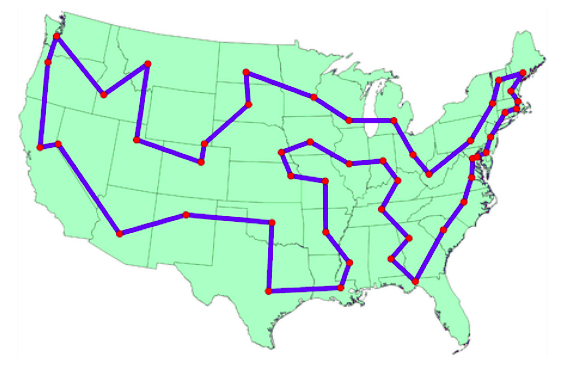
\includegraphics[width=0.5\textwidth]{commesso-viaggiatore.png}
    \caption{Esempio di soluzione per TSP}
\end{figure}

\begin{problem}[Copertura esatta di insiemi (EXACT-COVER)]
    Dati un insieme $X$ e una collezione $\mathcal{Y}=\{Y_1,\dots,Y_n\}$ di
    sottoinsiemi di $X$, dire se esiste una sottocollezione $\mathcal{Z}\subseteq
    \mathcal{Y}$ che partizioni $X$.
\end{problem}
\begin{eg}[Esempio di soluzione]
    Siano $X$ e $\mathcal{Y}$ definiti come segue:
    \[\begin{array}{lr}
        X=\{1,2,3,4,5,6,7\} & \mathcal{Y}=\{A,B,C,D,E,F\}
    \end{array}\]
    e siano gli elementi di $\mathcal{Y}$ i seguenti sottoinsiemi:
    \[\begin{array}{llllll}
        A=\{1,4,7\} & B=\{1,4\} & C=\{4,5,7\} & 
        D=\{3,5,6\} & E=\{2,3,6,7\} & F=\{2,7\}
    \end{array}\]
    Una partizione di $X$ è data da $\mathcal{Z}=\{B,D,F\}$. Un insieme
    $\mathcal{Z}$ è una partizione di $X$ in quanto $B\cap D\cap F=\emptyset$ e
    $B\cup D\cup F=X$.
\end{eg}

\begin{problem}[Partizione (PARTITION)]
    Dato un insieme $A$ contenente $n$ interi positivi, dire se esiste un
    sottoinsieme $S\subseteq\{1,\dots,n\}$ tale per cui $\sum_{i\in S}A[i]=
    \sum_{i\notin S}A[i]$.
\end{problem}

\begin{problem}[Somma di sottoinsieme (SUBSET-SUM)]
    Dati un vettore $A$ contenente $n$ interi positivi ed un intero positivo $k$,
    dire se esiste un sottoinsieme $S\subseteq\{1,\dots,n\}$ tale per cui
    $\sum_{i\in S}A[i]=k$.
\end{problem}

\begin{problem}[Zaino (KNAPSACK)]
    Dati un intero positivo $C$ e un insieme di $n$ oggetti tali per cui
    ciascun oggetto $i$ è caratterizzato da un peso $w[i]\in\mathbb{Z}$ e da un
    profitto $p[i]\in\mathbb{Z}$, dire se esiste un sottoinsieme $S\subseteq
    \{1,\dots,n\}$ tale che il peso totale $w(S)=\sum_{i\in S}w[i]\leq C$ e il
    profitto totale $p(S)=\sum_{i\in S}p[i]\geq k$ con $k\in\mathbb{Z}$.
\end{problem}

\begin{problem}[Circuito hamiltoniano (HAMILTONIAN-CIRCUIT)]
    Dato un grafo non orientato $G$, dire se esiste un cammino che attraversi
    ogni nodo una sola volta.
\end{problem}

\begin{figure}[h!]
\centering
\begin{graph}
    \tikzset{
        pos/.style args={#1:#2 from #3}{
          at=(#3.#1), anchor=#1+180, shift=(#1:#2)
        },
        point/.style={main, fill=red, minimum size=2mm, inner sep=0},
        empty/.style={inner sep=0}
    }

    \node[point] (0) {};
    \node[point] (1) [pos=-90+54:40mm from 0] {};
    \node[point] (2) [pos=-90-54:40mm from 0] {};
    \node[point] (3) [pos=36-108:40mm from 2] {};
    \node[point] (4) [pos=0:40mm from 3] {};

    \node[point] (5) [pos=-90:8.5mm from 0] {};
    \node[point] (6) [pos=-90-54:13mm from 5] {};
    \node[point] (7) [pos=36-180:13mm from 6] {};
    \node[point] (8) [pos=36-108:13mm from 7] {};
    \node[point] (9) [pos=108-180:13mm from 8] {};
    \node[point] (10) [pos=0:13mm from 9] {};
    \node[point] (11) [pos=0:13mm from 10] {};
    \node[point] (12) [pos=-180-108:13mm from 11] {};
    \node[point] (13) [pos=-108+180:13mm from 12] {};
    \node[point] (14) [pos=-90+54:13mm from 5] {};
    
    \node[point] (15) [pos=90:7.5mm from 10] {};
    \node[point] (16) [pos=90+54:11mm from 15] {};
    \node[point] (17) [pos=90-54:11mm from 15] {};
    \node[point] (18) [pos=-36+108:11mm from 16] {};
    \node[point] (19) [pos=0:11mm from 18] {};

    \draw[-, line width=1.3pt]
        (3) -- (2) -- (0) -- (1) -- (4) -- (11) -- (10) --
        (15) -- (16) -- (18) -- (19) -- (17) -- (12) -- (13) --
        (14) -- (5) -- (6) -- (7) -- (8) -- (9) -- (3);
    \draw[-, dashed]
        (3) -- (4)
        (9) -- (10)
        (6) -- (18)
        (14) -- (19)
        (15) -- (17)
        (0) -- (5)
        (1) -- (13)
        (2) -- (7)
        (11) -- (12)
        (8) -- (16);
\end{graph}
\caption{Esempio di \emph{circuito hamiltoniano}}
\end{figure}